\documentclass[printmode,pl]{mgr}

%opcje klasy dokumentu mgr.cls zostały opisane w dołączonej instrukcji, patrz plik <manual.pdf>

%poniżej deklaracje użycia pakietów, usunąć to co jest niepotrzebne
\usepackage{polski}       %przydatne podczas składania dokumentów w
%j. polskim 
%\usepackage[polish]{babel} %alternatywnie do pakietu
%polski, wybrać jeden z nich
%\usepackage[latin2]{inputenc} %kodowanie znaków, zależne od systemu
%\usepackage[T1]{fontenc} %poprawne składanie polskich czcionek

%pakiety do grafiki
\usepackage{graphicx}
\usepackage{subfigure}
\usepackage{psfrag}

%pakiety dodające dużo dodatkowych poleceń matematycznych
\usepackage{amsmath}
\usepackage{amsfonts}

%pakiety wspomagające i poprawiające składanie tabel
\usepackage{supertabular}
\usepackage{array}
\usepackage{tabularx}
\usepackage{hhline}

%pakiet wypisujący na marginesie etykiety równań i rysunków
%zdefiniowanych przez \label{}, chcąc wygenerować finalną wersję

\usepackage{showlabels}


\usepackage{microtype}


%definicje własnych poleceń
\newcommand{\R}{I\!\!R} %symbol liczb rzeczywistych, działa tylko w
                        %trybie matematycznym
\newtheorem{theorem}{Twierdzenie}[section] %nowe otoczenie do
                                           %składania twierdzeń

%dane do złożenia strony tytułowej
\title{Aplikacja webowa zwiększająca \\rozdzielczość obrazów}
\engtitle{Master thesis title}
\author{Eryk Wójcik}
\supervisor{dr hab. inż. Andrzej Rusiecki Prof. PWr}


%\guardian{dr hab. inż. Imię Nazwisko Prof. PWr} %nie używać
%jeśli opiekun jest tą samą osobą co prowadzący pracę

% \date{2023} %standardowo u dołu strony tytułowej umieszczany jest


%poniżej definiuje sie kierunek i ewentualną specjalność
%w obecnej wersji specjalność nie jest wypisywana na stronie tytułowej

\field{Automatyka i Robotyka (AIR)}
\specialisation{ART (ART)}

\begin{document}
\bibliographystyle{plabbrv} %tylko gdy używamy BibTeXa, ustawia polski styl bibliografii

\maketitle
% \dedication{6cm}{To jest przykładowa treść opcjonalnej dedykacji,
%   należy ją zmienić lub usunąć w całości polecenie
%   \texttt{$\backslash$dedication}}
\tableofcontents

\chapter{Wstęp}

W dobie cyfryzacji i rosnącej roli mediów wizualnych, jakość obrazu staje się kluczowym aspektem w wielu dziedzinach, zastosowania sięgają od rozrywki po medycynę. W odpowiedzi na te potrzeby, niniejsza praca inżynierska koncentruje się na opracowaniu aplikacji webowej, która wykorzystuje zaawansowane techniki przetwarzania obrazu w celu zwiększenia ich rozdzielczości.

Celem tej pracy jest zaprojektowanie i implementacja aplikacji, która z wykorzystaniem algorytmów DWSR \cite{guo2017deep} oraz ESRGAN \cite{wang2018esrgan} umożliwia znaczące polepszenie jakości obrazów. Wybór tych technologii podyktowany jest ich nowoczesnością i skutecznością.

% Motywacją do podjęcia tego tematu są rosnące potrzeby szerokiej dostępności narzędzi umożliwiających powiększanie rozdzielczości obrazów.

Celem pracy jest stworzenie nie tylko narzędzia do zwiększania rozdzielczości obrazów, ale przede wszystkim wdrożenie intuicyjnego interfejsu użytkownika umożliwiającego łatwe wykorzystanie algorytmów rozwiązujących problem super-rozdzielczości. W tym celu wykorzystane zostaną nowoczesne technologie webowe, które umożliwią dostęp do aplikacji z poziomu przeglądarki internetowej.

Układ pracy jest następujący. W rozdziale \ref{chap:podstawy_teoretyczne}. przedstawione zostały zagadnienia teoretyczne związane z tematem pracy. Kolejne rozdziały szczegółowo opisują zaimplementowane algorytmy: rozdział \ref{chap:DWSR}. opisuje algorytm DWSR, a rozdział \ref{chap:ESRGAN}. algorytm ESRGAN. Rozdział \ref{chap:app}. opisuje aplikację webową - narzędzie do porównywania wyników działania algorytmów. Rozdział \ref{chap:porownanie_algorytmow}. zawiera zestawienie zaimplementowanych metod. Rozdział \ref{chap:podsumowanie}. podsumowuje całość.
\chapter{Podstawy teoretyczne}

TODO: Napisz o k-means

Celem rozdziału jest przedstawienie podstawowych definicji, wytłumaczenie aparatu matematycznego oraz metod wykorzystywanych w algorytmach na których skupia się praca. Dodatkowo ma on na celu ułatwienie dalszego czytania poprzez zapoznanie czytelnika z przyjętymi konwencjami, oznaczeniami oraz symbolami, które mogą pojawić się w kolejnych rozdziałach. 


\section{Definicja super-rozdzielczości}

Super-rozdzielczość (ang. Super-Resolution) odnosi się do procesu poprawy rozdzielczości obrazu lub sekwencji obrazów. W kontekście cyfrowym, super-rozdzielczość jest często realizowana za pomocą algorytmów komputerowych, które mają na celu odtworzenie wysokiej rozdzielczości obrazu [Rys \ref{fig:image2}, \ref{fig:image3}] z jednego lub wielu obrazów o niskiej rozdzielczość [Rys \ref{fig:image1}].

\begin{figure}[ht]
    \centering
    \begin{minipage}[t]{0.3\linewidth}
        \includegraphics[width=\linewidth]{Rozdziały/02.Podstawy_teoretyczne/Obrazy/comic.png}
        \caption{Obraz oryginalny}
        \label{fig:image1}
    \end{minipage}
    \hspace{0.5cm}
    \begin{minipage}[t]{0.3\linewidth}
        \includegraphics[width=\linewidth]{Rozdziały/02.Podstawy_teoretyczne/Obrazy/comic_ESRGAN_x4.png}
        \caption{Obraz powiększony czterokrotnie}
        \label{fig:image2}
    \end{minipage}
    \hspace{0.5cm}
    \begin{minipage}[t]{0.3\linewidth}
        \includegraphics[width=\linewidth]{Rozdziały/02.Podstawy_teoretyczne/Obrazy/comic_ESRGAN_x16.png}
        \caption{Obraz powiększony szesnastokrotnie}
        \label{fig:image3}
    \end{minipage}
\end{figure}

\subsection*{Przykłady zastosowań super-rozdzielczości}

W kontekście praktycznym, techniki super-rozdzielczości znalazły zastosowanie w wielu dziedzinach. Przykładowo, w branży rozrywkowej, technika ta umożliwia remastering starych gier, filmów czy materiałów wideo do standardów HD czy 4K.

W ostatnich miesiącach popularne stało się generowanie obrazów z użyciem sztucznej inteligencji na podstawie podanego opisu tekstowego. Generowane w ten sposób obrazy są określonej wielkości i popularne modele takie jak \textbf{DALL-E} czy \textbf{Midjourney} nie pozwalają na zwiększenie jej. W tym miejscu z pomocą przychodzi super-rozdzielczość, która pozwala na powiększenie obrazów wygenerowanych w ten sposób.


\section{Przegląd metod powiększania obrazów}


Istnieje wiele metod powiększania rozdzielczości obrazów. Najprostszą z nich jest \textbf{interpolacja najbliższego sąsiada}, która polega na powieleniu pobliskich pikseli w celu zwiększenia rozdzielczości obrazu. \\
Metoda ta jest bardzo prosta w implementacji, jednakże nie daje ona zadowalających rezultatów. Obraz powiększony w ten sposób wygląda jak obraz o niskiej rozdzielczości z większymi pikselami [Rys \ref{fig:image5}]. 

\begin{figure}[ht]
    \centering
    \begin{minipage}[t]{0.32\linewidth}
        \includegraphics[width=\linewidth]{Rozdziały/02.Podstawy_teoretyczne/Obrazy/comic.png}
        \caption{Obraz oryginalny}
        \label{fig:image4}
    \end{minipage}
    \hspace{0.5cm}
    \begin{minipage}[t]{0.32\linewidth}
        \includegraphics[width=\linewidth]{Rozdziały/02.Podstawy_teoretyczne/Obrazy/comic_NN_x4.png}
        \caption{Obraz powiększony metodą najbliższego sąsiada}
        \label{fig:image5}
    \end{minipage}
  \end{figure}


Aby poprawić jakość obrazu, można zastosować \textbf{interpolację dwuliniową}. Metoda ta rozszerza interpolację liniową na interpolację funkcji dwóch zmiennych [Rys \ref{fig:image6}]. 

\begin{figure}[ht]
    \centering
    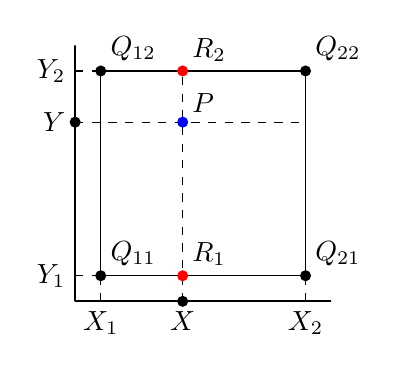
\begin{tikzpicture}[scale=1.3, dot/.style={circle,fill=black,minimum size=4pt,inner sep=0pt,outer sep=-1pt},]

        % Define the coordinates of the grid points
        \coordinate (A) at (1,1);
        \coordinate (B) at (3,1);
        \coordinate (C) at (1,3);
        \coordinate (D) at (3,3);

        \coordinate (R1) at (1.8,1);
        \coordinate (RY) at (1,2.5);
        \coordinate (R1end) at (1.8,3);
        \coordinate (RYend) at (3,2.5);

        \coordinate (P) at (1.8,2.5);

        \coordinate (X) at (1.8,0.75);
        \coordinate (Y) at (0.75,2.5);
        \coordinate (X1) at (1,0.75);
        \coordinate (X2) at (3,0.75);
        \coordinate (Y1) at (0.75,1);
        \coordinate (Y2) at (0.75,3);
        
        \coordinate (frameS) at (0.75,0.75);
        \coordinate (frameX) at (3.25,0.75);
        \coordinate (frameY) at (0.75,3.25);


        \draw[thick] (frameS) rectangle (frameX);
        \draw[thick] (frameS) rectangle (frameY);
        
        \draw[thin] (A) rectangle (D);
        
        % Draw lines from corners to the interpolated point
        \draw[dashed] (X) -- (R1end);
        \draw[dashed] (Y) -- (RYend);
        \draw[dashed] (X1) -- (A);
        \draw[dashed] (X2) -- (B);
        \draw[dashed] (Y1) -- (A);
        \draw[dashed] (Y2) -- (C);

        % Draw the dots
        \node[dot] at (A) {};
        \node[dot] at (B) {};
        \node[dot] at (C) {};
        \node[dot] at (D) {};
        \node[dot, blue] at (P) {};
        \node[dot, red] at (R1) {};
        \node[dot, red] at (R1end) {};
        \node[dot] at (X) {};
        \node[dot] at (Y) {};
        
        % Labels for the corners
        \node[above right] at (A) {$Q_{11}$};
        \node[above right] at (B) {$Q_{21}$};
        \node[above right] at (C) {$Q_{12}$};
        \node[above right] at (D) {$Q_{22}$};
        
        % Label for the interpolated point
        \node[above right] at (P) {$P$};

        \node[above right] at (R1) {$R_{1}$};
        \node[above right] at (R1end) {$R_{2}$};
        \node[below] at (X) {$X$};
        \node[left] at (Y) {$Y$};
        \node[below] at (X1) {$X_{1}$};
        \node[below] at (X2) {$X_{2}$};
        \node[left] at (Y1) {$Y_{1}$};
        \node[left] at (Y2) {$Y_{2}$};
        

        % Add title
        % \node[below] at (current bounding box.south) {Wizualizacja interpolacji dwuliniowej};

    \end{tikzpicture}
    
    \caption{Wizualizacja interpolacji dwuliniowej}
    \label{fig:image6}
\end{figure}


W efekcie polega to na wyznaczeniu średniej ważonej pikseli sąsiadujących z pikselem, który chcemy powielić. Współczynniki wag są wyznaczane na podstawie odległości od piksela, który chcemy powielić.
Kroki algorytmu:
\begin{enumerate}
    \item Przeprowadzana jest interpolacja liniowa wzdłuż osi $O X$:
    
    $$
    \begin{array}{llll}
    f\left(R_1\right) \approx \frac{x_2-x}{x_2-x_1} f\left(Q_{11}\right)+\frac{x-x_1}{x_2-x_1} f\left(Q_{21}\right) & \text { gdzie } & R_1=\left(x, y_1\right), \\ \\
    f\left(R_2\right) \approx \frac{x_2-x}{x_2-x_1} f\left(Q_{12}\right)+\frac{x-x_1}{x_2-x_1} f\left(Q_{22}\right) & \text { gdzie } & R_2=\left(x, y_2\right) .
    \end{array}
    $$
    \item Następnie przeprowadzana jest interpolacja wzdłuż osi $O Y$:
    $$
    f(P) \approx \frac{y_2-y}{y_2-y_1} f\left(R_1\right)+\frac{y-y_1}{y_2-y_1} f\left(R_2\right) .
    $$
\end{enumerate}


W efekcie otrzymujemy obraz wyglądający następująco [Rys \ref{fig:image8},  \ref{fig:image10}].


\begin{figure}[ht]
    \centering
    \begin{minipage}[t]{0.33\linewidth}
        \includegraphics[width=\linewidth]{Rozdziały/02.Podstawy_teoretyczne/Obrazy/bilinear_original.png}
        \caption{Obraz wejściowy}
        \label{fig:image7}
    \end{minipage}
    \hspace{0.5cm}
    \begin{minipage}[t]{0.33\linewidth}
        \includegraphics[width=\linewidth]{Rozdziały/02.Podstawy_teoretyczne/Obrazy/bilinear_enlarged.png}
        \caption{Obraz powiększony przez interpolację dwuliniową}
        \label{fig:image8}
    \end{minipage}
\end{figure}

\begin{figure}[ht]
    \centering
    \begin{minipage}[t]{0.33\linewidth}
        \includegraphics[width=\linewidth]{Rozdziały/02.Podstawy_teoretyczne/Obrazy/comic.png}
        \caption{Obraz wejściowy}
        \label{fig:image9}
    \end{minipage}
    \hspace{0.5cm}
    \begin{minipage}[t]{0.33\linewidth}
        \includegraphics[width=\linewidth]{Rozdziały/02.Podstawy_teoretyczne/Obrazy/comic_BILINEARx4.png}
        \caption{Obraz powiększony przez interpolację dwuliniową}
        \label{fig:image10}
    \end{minipage}
\end{figure}


Metoda ta daje lepsze rezultaty niż interpolacja najbliższego sąsiada, jednakże wprowadziła ona duże rozmycie, które jest szczególnie widoczne na krawędziach obiektów i obszarach wysokiej częstotliwości.



TODO: napisz o interpolacji dwusześciennej (bicubic)















\subsection*{Teoria informacji}

W teorii informacji istnieje koncepcja zwana \textbf{nierównością przetwarzania danych}. Zgodnie z nią niezależnie od sposobu przetwarzania danych, \textbf{nie można dodać informacji, której nie ma w oryginalnej serii danych}  [Wzór 2.1].

\begin{equation}
    \begin{gathered}
    X \rightarrow Y \rightarrow Z \\
    I(X ; Y) \geq I(X ; Z)
    \end{gathered}
\end{equation}

Oznacza to, że brakujących danych nie można odzyskać poprzez dalsze przetwarzanie. Czy to oznacza, że super-rozdzielczość jest teoretycznie niemożliwa? 

Nie, jeśli mamy dodatkowe źródło informacji. 


% \newpage

\section{Wprowadzenie do głębokiego uczenia się w przetwarzaniu obrazów}


Głębokie uczenie rewolucjonizuje przetwarzanie obrazów, wprowadzając modele zdolne do uczenia się cech z serii danych. W przetwarzaniu obrazów, głębokie sieci neuronowe są wykorzystywane do zadań takich jak detekcja obiektów, segmentacja, klasyfikacja obrazów, czy właśnie super-rozdzielczość [Rys \ref{fig:image12},  \ref{fig:image13}].

\begin{figure}[ht]
    \centering
    \begin{minipage}[t]{0.3\linewidth}
        \includegraphics[width=\linewidth]{Rozdziały/02.Podstawy_teoretyczne/Obrazy/comic.png}
        \caption{Obraz wejściowy}
        \label{fig:image11}
    \end{minipage}
    \hspace{0.5cm}
    \begin{minipage}[t]{0.3\linewidth}
        \includegraphics[width=\linewidth]{Rozdziały/02.Podstawy_teoretyczne/Obrazy/comic_DWSR_x4.png}
        \caption{Obraz powiększony algorytmem DWSR}
        \label{fig:image12}
    \end{minipage}
    \hspace{0.5cm}
    \begin{minipage}[t]{0.3\linewidth}
        \includegraphics[width=\linewidth]{Rozdziały/02.Podstawy_teoretyczne/Obrazy/comic_ESRGAN_x4.png}
        \caption{Obraz powiększony algorytmem ESRGAN}
        \label{fig:image13}
    \end{minipage}
\end{figure}

Sieć neuronowa może nauczyć się odtwarzać szczegóły obrazów na podstawie pewnych informacji, które zbiera z dużego zbioru obrazów. 

Szczegóły dodawane do powiększanego obrazu w przy użyciu modelu uczenia maszynowego nie naruszają nierówności przetwarzania danych, ponieważ wykorzystywane informacje są w zbiorze treningowym, nawet jeśli nie ma ich na obrazie wejściowym.


\subsection*{Podstawy Głębokiego Uczenia}
Głębokie uczenie, będące zaawansowaną formą uczenia maszynowego, wykorzystuje wielowarstwowe sieci neuronowe do analizy i interpretacji dużych zbiorów danych. Te sieci składają się z warstw skomplikowanych struktur algorytmicznych, które naśladują sposób, w jaki ludzki mózg przetwarza informacje.


\subsubsection*{Architektura Sieci Neuronowych}
Architektura sieci neuronowych w głębokim uczeniu charakteryzuje się wieloma ukrytymi warstwami, które pozwalają na przetwarzanie danych na różnych poziomach abstrakcji. Każda warstwa składa się z wielu neuronów, z których każdy otrzymuje dane wejściowe, przetwarza je i przekazuje dalej. Istnieją różne rodzaje warstw, w tym:
\begin{itemize}
    \item \textbf{Warstwy konwolucyjne (Convolutional Layers)}: Są fundamentem sieci konwolucyjnych (CNNs), które są szeroko stosowane w przetwarzaniu obrazów. Te warstwy stosują filtr konwolucyjny do danych wejściowych, wydobywając lokalne cechy, takie jak krawędzie, kształty czy tekstury.
    \item \textbf{Warstwy pooling (Pooling Layers)}: Redukują wymiarowość danych, jednocześnie zachowując ważne informacje. Najczęściej stosowanymi są max pooling i average pooling.
    \item \textbf{Warstwy w pełni połączone (Fully Connected Layers)}: Każdy neuron w tych warstwach jest połączony ze wszystkimi neuronami w poprzedniej warstwie, co pozwala na integrację nauczonej wiedzy z poprzednich warstw.
\end{itemize}


\subsubsection*{Funkcje Aktywacji}
Funkcje aktywacji w sieciach neuronowych to nieliniowe transformacje stosowane do wyjść neuronów. Pozwalają one na modelowanie złożonych zależności między danymi wejściowymi a wyjściowymi. W głębokim uczeniu stosuje się różne funkcje aktywacji, w tym:
\begin{itemize}
    \item \textbf{ReLU (Rectified Linear Unit)}: Przekształca wszystkie ujemne wartości na zero, podczas gdy wartości dodatnie pozostają niezmienione  [Rys \ref{fig:image14}].
    \item \textbf{Sigmoid}: Przyjmuje wartości wejściowe i konwertuje je na wartości z zakresu od 0 do 1 [Rys \ref{fig:image15}].
    \item \textbf{Tanh (Hyperbolic Tangent)}: Podobnie jak sigmoid, ale konwertuje wartości na zakres od -1 do 1 [Rys \ref{fig:image16}].
\end{itemize}

\begin{figure}[ht]
    \centering
    \begin{minipage}[t]{0.3\linewidth}
        \includegraphics[width=\linewidth]{Rozdziały/02.Podstawy_teoretyczne/Obrazy/relu.png}
        \caption{ReLU}
        \label{fig:image14}
    \end{minipage}
    \hspace{0.5cm}
    \begin{minipage}[t]{0.3\linewidth}
        \includegraphics[width=\linewidth]{Rozdziały/02.Podstawy_teoretyczne/Obrazy/sigmoid.png}
        \caption{Sigmoid}
        \label{fig:image15}
    \end{minipage}
    \hspace{0.5cm}
    \begin{minipage}[t]{0.3\linewidth}
        \includegraphics[width=\linewidth]{Rozdziały/02.Podstawy_teoretyczne/Obrazy/tanh.png}
        \caption{Tanh}
        \label{fig:image16}
    \end{minipage}
\end{figure}


\subsubsection*{Strategie Uczenia w Głębokim Uczeniu}
Głębokie uczenie obejmuje różne strategie uczenia, które są stosowane w zależności od rodzaju i charakteru danych oraz oczekiwanych wyników. Do głównych strategii należą:

\begin{itemize}
    \item \textbf{Uczenie nadzorowane (Supervised Learning)}: W tym podejściu model uczy się na podstawie zestawu danych, które zawierają zarówno dane wejściowe, jak i odpowiednie etykiety. Jest to szeroko stosowane w zadaniach takich jak np. klasyfikacja.
    \item \textbf{Uczenie nienadzorowane (Unsupervised Learning)}: Model próbuje znaleźć wzorce w danych bez etykiet, stosowane głównie w grupowaniu i redukcji wymiarowości.
    \item \textbf{Uczenie ze wzmacnianiem (Reinforcement Learning)}: W tej strategii agent uczy się podejmować decyzje poprzez interakcje z otoczeniem, dążąc do maksymalizacji sumy nagród.
\end{itemize}


\subsubsection*{Przeuczenie i Generalizacja}

Przeuczenie (Overfitting) występuje, gdy model zbyt dokładnie dopasowuje się do danych treningowych, tracąc zdolność do efektywnego działania na nowych danych [Rys \ref{fig:image17}]. Niebieska linia reprezentuje przeuczony model, zaś czarna dopasowany. Widać że niebieska linia podąża za danymi treningowymi, jest zbyt zależna od nich co sprawia, że model przeuczony będzie miał wyższy poziom błędu dla nowych danych. Jest to problem szczególnie w przypadku zbyt skomplikowanych modeli w stosunku do danych.
\begin{figure}[h]
    \centering
    \includegraphics[width=0.4\linewidth]{Rozdziały/02.Podstawy_teoretyczne/Obrazy/overfitting.png}
    \caption{Wizualizacja przeuczenia}
    \label{fig:image17}
\end{figure}

Celem jest stworzenie modelu, który efektywnie działa na nowych, nieznanych danych, co oznacza, że model jest dobrze dostosowany do rzeczywistych scenariuszy.

Przykładowe sposoby na zapobieganie przeuczeniu:

\begin{itemize}
    \item \textbf{Wczesne zatrzymywanie (early stopping):} Polega na monitorowaniu wydajności modelu na zestawie walidacyjnym i zatrzymaniu treningu, gdy wydajność przestaje się poprawiać, co zapobiega przeuczeniu.
    \item \textbf{Walidacja krzyżowa (cross-validation):} Metoda oceny modelu, w której zestaw danych dzieli się na kilka części. Model jest następnie trenowany na jednej części (zwanej zestawem treningowym) i walidowany na innej (zwanej zestawem walidacyjnym), co jest powtarzane na różnych kombinacjach części danych. Pozwala to na lepszą ocenę zdolności modelu do generalizacji na nieznanych danych.s
    \item \textbf{Augmentacja danych (data augmentation):} Zwiększa różnorodność danych treningowych poprzez wprowadzenie niewielkich losowych zmian, co pomaga modelowi lepiej uogólnić i zmniejszyć przeuczenie.
\end{itemize}


\subsubsection*{Generatywne Sieci Przestawne}

Generatywne sieci przestawne (ang: \textit{Generative Adversarial Networks}) to rodzaj architektury sieci neuronowej, która składa się z dwóch sieci: generatora i dyskryminatora. Generator próbuje wygenerować dane, które są podobne do danych treningowych, podczas gdy dyskryminator próbuje stwierdzić prawdopodobieństwo, że dane pochodzą z danych treningowych, a nie z generatora.
Sposób ten wywodzi się z teorii gier, gdzie agenci grają przeciw sobie. W tym przypadku rolą generatora jest oszukiwanie dyskryminatora, podczas gry rolą dyskryminatora jest nie dać się oszukać. 

Te dwie sieci są trenowane naprzemiennie, aż do osiągnięcia równowagi, w której dyskryminator nie jest w stanie odróżnić danych wygenerowanych przez generator od danych treningowych, w wyniku czego dyskryminator zawsze zwracaja prawdopodobieństwo równe $0.5$.
Ciekawą rzeczą w generatywnych sieciach jest to, że model musi pracować bardziej, gdy zawodzi. Dyskryminator szuka słabości generatora i zmusza go do poprawy, zaś generator adresuje te problemy. Gdy generator naprawi swoje błędy, dyskryminator szuka kolejni słabości, co prowadzi do ciągłego rozwoju obu sieci.

% W generatywnych sieciach przestawnych 

% \begin{figure}[h]
%     \centering
%     \includegraphics[width=0.7\linewidth]{Rozdziały/02.Podstawy_teoretyczne/Obrazy/generator_dyskryminator.png}
%     \caption{Funkcje strat generatora i dyskryminatora}
%     \label{fig:image59}
% \end{figure}

\subsection*{Algorytmy Głębokiego Uczenia w Super-Rozdzielczości}

Aby stworzyć algorytm głębokiego uczenia do zastosowania w problemie Super-Rozdzielczości potrzebujemy zestawu danych z obrazami o wysokiej rozdzielczości i tych samych obrazów ze zmniejszoną rozdzielczością.

Następnie trenujemy model, który jako wejście przyjmuje obraz o niskiej rozdzielczości i zwraca obraz o wysokiej rozdzielczości, który jest najbliższy oryginałowi.


\begin{figure}[h]
    \centering
    \includegraphics[width=0.55\linewidth]{Rozdziały/02.Podstawy_teoretyczne/Obrazy/SR_CNN.png}
    \caption{Przykład sieci neuronowej do super-rozdzielczości}
    \label{fig:image18}
\end{figure}



Do porównania obrazu wyjściowego z obrazem oryginalnym można wykorzystać funkcję błędu średniokwadratowego \textit{MSE - Mean Squared Error}, która jest zdefiniowana jako średnia arytmetyczna kwadratów różnic między wartościami pikseli w obrazie wyjściowym $\hat{\theta }$ i oryginalnym $\theta$ [Równanie \ref{eq:1}].

\begin{equation}
    MSE(\hat{\theta }) = \sum(\hat{\theta } - \theta )^2 \label{eq:1}
\end{equation}

Ale czy metoda błędu średniokwadratowego jest odpowiednia do optymalizacji?
Niestety błąd średniokwadratowy nie wyraża dobrze ludzkiego postrzegania wierności obrazu \cite{4775883}.

\begin{figure}[h]
    \centering
    \includegraphics[width=0.55\linewidth]{Rozdziały/02.Podstawy_teoretyczne/Obrazy/MSE.png}
    \caption{Przykład sieci neuronowej do super-rozdzielczości}
    \label{fig:image56}
\end{figure}

Przykładowo wszystkie obrazy na Rysunku \ref{fig:image56} mają ten sam błąd średniokwadratowy, ale różnią się znacząco wizualnie. W tym przypadku błąd średniokwadratowy nie jest w stanie wykryć różnic w jakości obrazu. 

Metoda błędu średniokwadratowego nie bierze pod uwagę różnic strukturalnych między obrazami, z tego wynikają różnice przedstawione wyżej.

Rozwiązaniem tego może być inna miara błędu, która bierze pod uwagę różnice strukturalne między obrazami. Jedną z takich miar jest \textbf{błąd strukturalny} \textit{SSIM - Structural Similarity Index Measure} \cite{1284395}, który jest zdefiniowany jako funkcja zależna od obrazu, która mierzy podobieństwo między dwoma obrazami. SSIM jest zdefiniowany jako iloczyn trzech funkcji: podobieństwa jasności, kontrastu i struktury [Równanie \ref{eq:2}].

\begin{equation}
    SSIM(x,y) = [l(x,y)][c(x,y)][s(x,y)] \label{eq:2}
\end{equation}


\newpage

\section{Wstęp do transformacji falkowej}


Transformacja falkowa (wavelet transform) stanowi istotne narzędzie w analizie sygnałów i przetwarzaniu obrazów, zwłaszcza w kontekście zastosowań takich jak super rozdzielczość. Charakterystyczna dla funkcji falkowych jest ich zdolność do dostosowania się do wymagań analizy sygnału. W przeciwieństwie do transformacji Fouriera, która skupia się wyłącznie na częstotliwości, falki pozwalają na efektywną lokalizację zjawisk w sygnale, uwzględniając zmiany zarówno w czasie, jak i częstotliwości.

\begin{figure}[ht]
    \centering

    \begin{minipage}[t]{0.3\linewidth}
        \includegraphics[width=\linewidth]{Rozdziały/02.Podstawy_teoretyczne/Obrazy/horizontal_detail.png}
        \caption{Detale poziome}
        \label{fig:image19}
    \end{minipage}
    \hspace{0.5cm}
    \begin{minipage}[t]{0.3\linewidth}
        \includegraphics[width=\linewidth]{Rozdziały/02.Podstawy_teoretyczne/Obrazy/vertical_detail.png}
        \caption{Detale pionowe}
        \label{fig:image20}
    \end{minipage}
    \hspace{0.5cm}
    \begin{minipage}[t]{0.3\linewidth}
        \includegraphics[width=\linewidth]{Rozdziały/02.Podstawy_teoretyczne/Obrazy/diagonal_detail.png}
        \caption{Detale diagonalne}
        \label{fig:image21}
    \end{minipage}
\end{figure}\

W kontekście super rozdzielczości, funkcje falkowe są wykorzystywane do zwiększania jakości obrazów i sygnałów poprzez umożliwienie dokładniejszej analizy i rekonstrukcji ich składowych. Mamy informacje o kierunkach i wielkościach częstotliwości w analizowanym obrazie [Rys \ref{fig:image19}, \ref{fig:image20} \ref{fig:image21}]. 
% Korzystając z funkcji falkowych mamy informacje o kierunkach częstotliwości w analizowanym obrazie, co sprawia że wiemy jak ukierunkowane są krawędzie i tekstury. 
% Dzięki swoim właściwościom, falki potrafią efektywnie oddzielać istotne cechy sygnału od szumu, co jest istotne w procesie zwiększania rozdzielczości.


\subsubsection{Dziedzina czasu i częstotliwości}

Dziedzina czasu odnosi się do analizy sygnału w zakresie czasu, co oznacza, że sygnał jest przedstawiany i analizowany w kontekście jego zmian w czasie. Jest to intuicyjna forma reprezentacji sygnałów, niemniej jednak nie daje ona nam pełnej informacji o sygnale. Z drugiej strony sygnał możemy określić w dziedzinie częstotliwości, która koncentruje się na analizie częstotliwościowych składników sygnału.

% W przetwarzaniu obrazów dziedzina częstotliwości jest często stosowana na przykład do usuwania szumów, wykrywania wzorców i stosowania różnych filtrów.

\begin{figure}[h]
    \centering
    \includegraphics[width=0.47\linewidth]{Rozdziały/02.Podstawy_teoretyczne/Obrazy/time-frequency-domain.png}
    \caption{Wizualizacja dziedziny czasu i częstotliwości}
    \label{fig:image22}
\end{figure}



\subsection*{Transformata Fouriera}

Transformacja Fouriera jest algorytmem używanym do konwersji sygnału z dziedziny czasu do dziedziny częstotliwości. Pozwala ona na uzyskanie widma amplitudowego i fazowego, które prezentują częstotliwości występujące w sygnale i ich amplitudy.

\begin{figure}[h]
    \centering
    \includegraphics[width=0.8\linewidth]{Rozdziały/02.Podstawy_teoretyczne/Obrazy/fft.png}
    \caption{Wynik transformacji Fouriera dla przykładowego sygnału}
    \label{fig:image23}
\end{figure}

W kontekście przetwarzania obrazów, transformata Fouriera jest stosowana przekształcenia obrazu do dziedziny częstotliwościowej. Wynik transformacji Fouriera jest liczbą zespoloną, która może być reprezentowana jako wektor złożony z dwóch części: rzeczywistej i urojonej, co być przedstawione w postaci dwóch wykresów: amplitudowego i fazowego [Rys \ref{fig:image25}, \ref{fig:image26}].

\begin{figure}[ht]
    \centering
    \begin{minipage}[t]{0.325\linewidth}
        \includegraphics[width=\linewidth]{Rozdziały/02.Podstawy_teoretyczne/Obrazy/comic_DWSR_x4.png}
        \caption{Obraz wejściowy}
        \label{fig:image24}
    \end{minipage}
    % \hspace{0.5cm}
    \begin{minipage}[t]{0.325\linewidth}
        \includegraphics[width=\linewidth]{Rozdziały/02.Podstawy_teoretyczne/Obrazy/fft_magnitude.png}
        \caption{Wykres amplitudowy}
        \label{fig:image25}
    \end{minipage}
    % \hspace{0.5cm}
    \begin{minipage}[t]{0.325\linewidth}
        \includegraphics[width=\linewidth]{Rozdziały/02.Podstawy_teoretyczne/Obrazy/fft_phase.png}
        \caption{Wykres fazowy}
        \label{fig:image26}
    \end{minipage}
\end{figure}\

Transformacja Fouriera jest operacją odwracalną, co oznacza, że można ją wykorzystać do rekonstrukcji oryginalnego sygnału z częstotliwościowej reprezentacji stosując odwrotną transformację Fouriera.


\subsubsection{Ograniczenia Transformacji Fouriera}

Zgodnie z zasadą nieoznaczoności Heisenberga nie można jednocześnie precyzyjnie określić i lokalizować zjawisk zarówno w dziedzinie czasu, jak i częstotliwości, zawsze mamy do czynienia z kompromisem. 
\begin{equation}
    \Delta f \Delta t \geq 1
\end{equation}
Możemy albo dokładnie określić wartość sygnału w czasie, albo dokładnie określić jego częstotliwość, ale nie możemy zrobić obu jednocześnie.

W rezultacie, podczas gdy Transformata Fouriera oferuje doskonałą rozdzielczość częstotliwościową, traci na zdolności do lokalizacji zjawisk w czasie. Oznacza to, że badając sygnał wyłącznie w dziedzinie częstotliwości, wiemy jakie częstotliwości występują, ale nie jesteśmy w stanie określić kiedy występuje dana częstotliwość.

Czy istnieje narzędzie pozwalające nam na dokładniejszą analizę sygnału? Kompromis pomiędzy czasem a częstotliwością jest nieunikniony, ale istnieje sposób na poprawę lokalizacji w czasie kosztem rozdzielczości częstotliwościowej? Odpowiedzią na te pytania jest transformacja falkowa.


\subsection*{Funkcje Falkowe}

Gdy wykonujemy transformatę Fouriera rozdzielamy sygnał na sumę sinusoid i cosinusoid o różnych częstotliwościach. Funkcje falkowe są podobne do funkcji sinusoidalnych, ale różnią się od nich tym, że mają skończoną długość i są ograniczone do określonego obszaru [Rys \ref{fig:image27}, \ref{fig:image28}].

\begin{figure}[ht]
    \centering
    \begin{minipage}[t]{0.45\linewidth}
        \includegraphics[width=\linewidth]{Rozdziały/02.Podstawy_teoretyczne/Obrazy/sine_wave.png}
        \caption{Sinusoida}
        \label{fig:image27}
    \end{minipage}
    \hspace{0.5cm}
    \begin{minipage}[t]{0.45\linewidth}
        \includegraphics[width=\linewidth]{Rozdziały/02.Podstawy_teoretyczne/Obrazy/morlet_wavelet.png}
        \caption{Falka Morlet}
        \label{fig:image28}
    \end{minipage}
\end{figure}


Funkcje falkowe są rodziną funkcji. Aby funkcja $\Psi(t)$ była falką, musi spełniać następujące warunki:
\begin{itemize}
    \item Funkcja musi mieć zerową średnią, czyli całka z funkcji musi być równa 0 (powierzchnia poniżej krzywej musi być równa powierzchni powyżej krzywej):
        \begin{equation}
            \int_{-\infty}^{+\infty} \Psi(t) d t=0
        \end{equation}
    \item Funkcja musi mieć skończoną energię (to ograniczenie sprawia, że funkcja jest ograniczona do określonego obszaru):
        \begin{equation}
            \int_{-\infty}^{+\infty}|\Psi(t)|^{2} d t<\infty
        \end{equation}
\end{itemize}

Przykładem może być falka Morlet, która jest jedną z najczęściej stosowanych funkcji falkowych. Falka Morlet jest funkcją sinusoidalną, która jest przemnożona przez funkcję Gaussa. Rzeczywista część falki Morlet jest zdefiniowana następująco:
\begin{equation}
    \Psi(t)=k_0 \cdot \cos (\omega t) \cdot e^{-\frac{t^2}{2}}
\end{equation}

Część rzeczywista Morlet składa się funkcji cosinus (określająca częstotliwość falki) i funkcji Gaussa, która jest odpowiedzialna za ograniczenie falki do określonego obszaru.

\begin{figure}[ht]
    \centering
    \begin{minipage}[t]{0.7\linewidth}
        \includegraphics[width=\linewidth]{Rozdziały/02.Podstawy_teoretyczne/Obrazy/morlet_e}
        \caption{Falka Morlet (część rzeczywista)}
        \label{fig:image29}
    \end{minipage}
\end{figure}

Falka Morlet jest funkcją zespoloną, co oznacza, że składa się z części rzeczywistej i urojonej. Całość jest zdefiniowana następująco:
\begin{equation}
    \Psi(t)=k e^{i \omega_0 t} \cdot e^{-\frac{t^2}{2}}
\end{equation}

\begin{figure}[ht]
    \centering
    \begin{tikzpicture}[scale=0.8]
        \begin{axis}[
          ylabel={Re($\Psi$)},
          zlabel={Im($\Psi$)},
          xlabel={Czas},
          view={155}{30},
          colormap/viridis,
        ]
        \addplot3+[mesh, samples=30] table {Rozdziały/02.Podstawy_teoretyczne/Obrazy/wave_data.txt}; % Wczytanie danych
        \end{axis}
    \end{tikzpicture}
    \caption{Falka Morlet w przestrzeni 3D}
    \label{fig:image30}
\end{figure}

Inne funkcje falkowe:

\begin{figure}[ht]
    \centering
    \begin{minipage}[t]{0.3\linewidth}
        \includegraphics[width=\linewidth]{Rozdziały/02.Podstawy_teoretyczne/Obrazy/wavelet_fbsp1-1.5-1.0.png}
        \caption{Falka fbsp}
        \label{fig:image31}
    \end{minipage}
    \hspace{0.5cm}
    \begin{minipage}[t]{0.3\linewidth}
        \includegraphics[width=\linewidth]{Rozdziały/02.Podstawy_teoretyczne/Obrazy/wavelet_mexh.png}
        \caption{Falka Mexican Hat}
        \label{fig:image32}
    \end{minipage}
    \hspace{0.5cm}
    \begin{minipage}[t]{0.3\linewidth}
        \includegraphics[width=\linewidth]{Rozdziały/02.Podstawy_teoretyczne/Obrazy/wavelet_gaus1.png}
        \caption{Falka Gaussa}
        \label{fig:image33}
    \end{minipage}
\end{figure}


\subsection*{Transformacja Falkowa}

Transformacja falkowa to proces dekompozycji sygnału na zestaw funkcji falkowych. W przeciwieństwie do transformacji Fouriera, która analizuje sygnał w kontekście czystych częstotliwości, transformacja falkowa rozkłada sygnał na serię "falek", które są przesuwane w czasie i częstotliwości, aby zbadać charakterystykę sygnału.


Transformację falkową przedstawiamy jako:

\begin{equation}
    \tilde{s}_{\Psi}(a, b)=\frac{1}{\sqrt{a}} \int_{-\infty}^{\infty} s(t) \Psi\left(\frac{t-b}{a}\right) \mathrm{dt},
\end{equation}

gdzie:
\begin{itemize}
    \item $s(t)$ - sygnał wejściowy,
    \item $\Psi\left(\frac{t-b}{a}\right)$ - funkcja falkowa,
    \item $b$ - parametr przesunięcia (w dziedzinie czasu) [Rys \ref{fig:image35}].
    \item $a$ - parametr skali (przesunięcie w dziedzinie częstotliwości) [Rys \ref{fig:image36}],
\end{itemize}


\begin{figure}[ht]
    \centering
    \begin{minipage}[t]{0.47\linewidth}
        \includegraphics[width=\linewidth]{Rozdziały/02.Podstawy_teoretyczne/Obrazy/morlet_bez_przesuniecia.png}
        \caption{Brak przesunięcia}
        \label{fig:image34}
    \end{minipage}
    \centering
    \begin{minipage}[t]{0.47\linewidth}
        \includegraphics[width=\linewidth]{Rozdziały/02.Podstawy_teoretyczne/Obrazy/time_shift_morlet.png}
        \caption{Przesunięcie w czasie}
        \label{fig:image35}
    \end{minipage}
\end{figure}

\begin{figure}[ht]
    \centering
    \begin{minipage}[t]{0.46\linewidth}
        \includegraphics[width=\linewidth]{Rozdziały/02.Podstawy_teoretyczne/Obrazy/f_shift_morlet.png}
        \caption{Przesunięcie w częstotliwości}
        \label{fig:image36}
    \end{minipage}
    \centering
    \begin{minipage}[t]{0.46\linewidth}
        \includegraphics[width=\linewidth]{Rozdziały/02.Podstawy_teoretyczne/Obrazy/t_and_f_shift_morlet.png}
        \caption{Przesunięcie w $t$ i $f$}
        \label{fig:image37}
    \end{minipage}
\end{figure}


Wynikiem transformacji falkowej jest mapa współczynników, które są zależne od parametrów $a$ i $b$, wybranej funkcji falkowej oraz sygnału wejściowego. Dla danych wartości $a$ i $b$ współczynnik jest miarą podobieństwa pomiędzy falką a fragmentem sygnału. Im większa wartość współczynnika, tym większe podobieństwo.

% \begin{equation}
%     T\left(a,b\right) = \int_{-\infty}^{+\infty} y(t) \cdot \Psi_{a, b}(t) d t
% \end{equation}

W rezultacie funkcja $ \tilde{s}_{\Psi}\left(a,b\right)$ składa się na mapę współczynników, która jest reprezentacją sygnału w dziedzinie czasu i częstotliwości. Mapę taką nazywamy skalogramem, skalogram przykładowego sygnału przedstawiono na Rys \ref{fig:image38} i \ref{fig:image39}.

\begin{figure}[ht]
    \centering
    \begin{minipage}[t]{0.9\linewidth}
        \includegraphics[width=\linewidth]{Rozdziały/02.Podstawy_teoretyczne/Obrazy/skalogram.png}
        \caption{Skalogram falkowy w zestawieniu z sygnałem wejściowym}
        \label{fig:image38}
    \end{minipage}
\end{figure}

\begin{figure}[ht]
    \centering
    \begin{tikzpicture}[scale=0.95]
        \begin{axis}[
          xlabel={Czas},
          ylabel={Częstotliwość},
          zlabel={Amplituda},
          view={-40}{40},
          colormap/viridis,
          yticklabel=\empty,            % Hide y-axis numbers
          xticklabel=\empty,            % Hide x-axis numbers
          zticklabel=\empty,            % Hide z-axis numbers
        ]
        \addplot3[surf] file {Rozdziały/02.Podstawy_teoretyczne/Obrazy/wavelet_coefficients_magnitude.txt};
        \end{axis}
    \end{tikzpicture}
    \caption{Skalogram falkowy w przestrzeni 3D}
    \label{fig:image39}
\end{figure}
\newpage
Rozdzielczość czasu i rozdzielczości w transformacji falkowej nie jest idealna, widać że mamy do czynienia z kompromisem pomiędzy tymi wartościami, szczególnie przy analizy zwykłej funkcji sinus. Skalogram dla sinusa [Rys \ref{fig:image40}] nie przedstawia jednoznacznie częstotliwości sygnału, jest to jedynie przybliżenie co widać na krawędziach skalogramu.

\begin{figure}[ht]
    \centering
    \begin{minipage}[t]{0.55\linewidth}
        \includegraphics[width=\linewidth]{Rozdziały/02.Podstawy_teoretyczne/Obrazy/skalogram_sinus.png}
        \caption{Niedokładność danych na skalogramie}
        \label{fig:image40}
    \end{minipage}
\end{figure}

\newpage
\subsubsection{Dyskretna Transformacja Falkowa}

Dyskretna transformacja falkowa (DWT) jest dyskretną wersją transformacji falkowej, czyli działa na dyskretnych danych wejściowych. Przykładem takich danych może być cyfrowy sygnał taki jak obraz lub dźwięk. 

Dla sygnałów dyskretnych, transformacja falkowa jest zdefiniowana jako:
\begin{equation}
    \mathrm{D}\left(m, a^j\right)=\frac{1}{\sqrt{a^j}} \sum_{n=0}^{N-1} x\varphi^*[n] \left(\frac{n-m}{a^j}\right),
\end{equation}
gdzie:
\begin{itemize}
    \item $x[n]$ - sygnał dyskretny,
    \item $\varphi[n]$ - dyskretna funkcja falkowa,
    \item $a$ - parametr skali,
    \item $j$ - poziom dekompozycji,
    \item $N$ - liczba próbek sygnału,
    \item $m$ - indeks próbki.
\end{itemize}

Aby wykonać dyskretną transformację falkową sygnał $x[n] \in \mathbb{R}^N$ jest przepuszczany przez filtr górnoprzepustowy $G_H[n]$ i filtr dolnoprzepustowy $G_L[n]$, które są definiowane jako (w przypadku falki Haara):

\begin{equation}
    G_H[n]=\left\{\begin{array}{ll}
    1, & n=0 \\
    -1, & n=1 \\
    0, & \text {w przeciwnym razie}
    \end{array}, 
    G_L[n]= \begin{cases}1, & n=0,1 \\
    0, & \text {w przeciwnym razie}\end{cases}\right.
\end{equation}

Po filtrowaniu połowa próbek może zostać wyeliminowana zgodnie z regułą Nyquista, ponieważ sygnał ma teraz pasmo częstotliwości $\frac{\pi}{2}$ radianów zamiast $/pi$.

Obraz $x$ jest reprezentowany jako sygnał $2 D$ o indeksach $[n,m]$, gdzie $x[n,m]$ jest wartością piksela w $n$-tej kolumnie i $m$-tym wierszu.

Sygnał dwuwymiarowy $x[n,m]$ może być traktowany jako dwa sygnały jednej zmiennej: $x[n,:]$ w $n$-tej kolumnie i wśród kolumn $x[:,m]$ w $m$-tym wierszu. Transformacja falkowa o pierwszym stopniu dekompozycji może być wykonywana w sposób przedstawiony na Rys \ref{fig:image41}.

\begin{figure}[ht]
    \centering
    \begin{minipage}[t]{0.6\linewidth}
        \includegraphics[width=\linewidth]{Rozdziały/02.Podstawy_teoretyczne/Obrazy/DWT_dekompozycja.png}
        \caption{Dekompozycja DWT 1-poziomu}
        \label{fig:image41}
    \end{minipage}
\end{figure}

Przykładowa dekompozycja pierwszego stopnia wykonana na obrazie \textbf{comic.png} widoczna jest na Rys \ref{fig:image42} - niskie częstotliwości na obrazie, \ref{fig:image43} - poziome detale, \ref{fig:image44} - pionowe detale, \ref{fig:image45} - detale diagonalne. Obrazy po dekompozycji są tej samej wielkości co obraz wejściowy. 

Jeśli chcemy wykonać odwrotną transformację falkową na obrazie, wystarczy wykonać kroki z Rys \ref{fig:image41}. 


\begin{figure}[ht]
    \centering
    \begin{minipage}[t]{0.35\linewidth}
        \includegraphics[width=\linewidth]{Rozdziały/02.Podstawy_teoretyczne/Obrazy/level_1_decomposition_LL.png}
        \caption{LL (niskie częstotliwości)}
        \label{fig:image42}
    \end{minipage}
    \centering
    \begin{minipage}[t]{0.35\linewidth}
        \includegraphics[width=\linewidth]{Rozdziały/02.Podstawy_teoretyczne/Obrazy/level_1_decomposition_LH.png}
        \caption{LH (poziome detale)}
        \label{fig:image43}
    \end{minipage}
\end{figure}

\begin{figure}[ht]
    \centering
    \begin{minipage}[t]{0.35\linewidth}
        \includegraphics[width=\linewidth]{Rozdziały/02.Podstawy_teoretyczne/Obrazy/level_1_decomposition_HL.png}
        \caption{HL (pionowe detale)}
        \label{fig:image44}
    \end{minipage}
    \centering
    \begin{minipage}[t]{0.35\linewidth}
        \includegraphics[width=\linewidth]{Rozdziały/02.Podstawy_teoretyczne/Obrazy/level_1_decomposition_HH.png}
        \caption{HH (diagonalne detale)}
        \label{fig:image45}
    \end{minipage}
\end{figure}

\chapter{Deep Wavelet Super Resolution}


Pierwszy z omawianych algorytmów adresuje problem super-rozdzielczości obrazów przy użyciu transformacji falkowej i głębokiej sieci neuronowej. Algorytm został opracowany przez: Tiantong Guo, Hojjat Seyed Mousavi, Tiep Huu Vu, Vishal Monga, dla: School of Electrical Engineering and Computer Science, The Pennsylvania State University, State College, PA, 16803 \cite{guo2017deep}.
Ta głęboka sieć neuronowa skupia się na rekonstrukcji różnic pomiędzy obrazkiem wejściowym o niskiej rozdzielczości (LR - Low Res), a obrazkiem wysokiej rozdzielczości (HR - High Res). W tej pracy badane są zalety wykorzystywania danych domeny transformacji falkowej w zadaniu SR, zwłaszcza w celu uchwycenia większej ilości informacji strukturalnych w obrazach aby uniknąć artefaktów. 

Rezydualne sieci neuronowe korzystają z nieliczności danych wejściowych i wyjściowych oraz faktu, że uczenie sieci z nielicznymi aktywacjami jest znacznie łatwiejsze i bardziej niezawodne. 
To pozwala na wykorzystanie przestrzennych współczynników falkowych, które zazwyczaj są rzadkie. Co ważniejsze, wykorzystanie różnic współczynników falkowych jako par danych treningowych dodatkowo zwiększa rzadkość danych treningowych, co skutkuje bardziej efektywnym uczeniem. Innymi słowy, użycie współczynników falkowych sprzyja rzadkości aktywacji w warstwach środkowych, a także w warstwie wyjściowej.

\begin{figure}[ht]
    \centering
    \begin{minipage}[t]{0.35\linewidth}
        \includegraphics[width=\linewidth]{Rozdziały/02.Podstawy_teoretyczne/Obrazy/comic.png}
        \caption{Obraz wejściowy}
        \label{fig:image46}
    \end{minipage}
    \hspace{0.5cm}
    \begin{minipage}[t]{0.35\linewidth}
        \includegraphics[width=\linewidth]{Rozdziały/02.Podstawy_teoretyczne/Obrazy/comic_DWSR_x4.png}
        \caption{Obraz powiększony algorytmem DWSR czterokrotnie}
        \label{fig:image47}
    \end{minipage}
\end{figure}

Dodatkowo transformacja falkowa dekomponuje obraz na wiele skal, co pozwala na wykorzystanie informacji z różnych skal w celu rekonstrukcji obrazu o wysokiej rozdzielczości. W przeciwieństwie do innych metod, które wykorzystują informacje z jednej skali, DWSR wykorzystuje informacje z wielu skal, co pozwala na lepsze odwzorowanie obrazu o wysokiej rozdzielczości.


\section{Architektura DWSR}

Na problem super-rozdzielczości mozemy spojrzeć jak na problem rekonstrukcji detali w obrazie wejściowym o niskiej rozdzielczości. Takie podejście świetnie współgra z dekompozycją transformacji falkowej. Jak widać na Rys \ref{fig:image48}, jeśli potraktujemy obraz wejściowy jako wyjście LL poziomu 2dDWT, przewidywanie podpasm HL, LH i HH 2dDWT da nam brakujące szczegóły obrazu LL. Następnie można użyć 2dIDWT, aby zebrać przewidywane szczegóły i wygenerować wyniki SR.


\begin{figure}[ht]
    \centering
    \begin{minipage}[t]{0.7\linewidth}
        \includegraphics[width=\linewidth]{Rozdziały/03.DWSR/Obrazy/konstrukcja_2dDWT.png}  
        \caption{Proces dekompozycji Dyskretnej Transformacji Falkowej}
        \label{fig:image48}
    \end{minipage}
\end{figure}


Korzystając z falki Haar, współczynniki 2dDWT można zapisać jako:
\begin{equation*}
    \left\{\begin{array}{l}
    A=a+b+c+d \\
    B=a-b+c-d \\
    C=a+b-c-d \\
    D=a-b-c+d
    \end{array}\right.
\end{equation*}
gdzie: 
\begin{itemize}
    \item $A, B, C, D$ są pikselami zlokalizowanymi w siatce $2 \times  2$ w lewym górnym rogu obrazu HR,
    \item $a$ jest pikselem zlokalizowanym w lewym górnym rogu obrazu LL,
    \item $b$ jest pikselem zlokalizowanym w lewym górnym rogu obrazu HL,
    \item $c$ jest pikselem zlokalizowanym w lewym górnym rogu obrazu LH,
    \item $d$ jest pikselem zlokalizowanym w lewym górnym rogu obrazu HH.
\end{itemize}

Dlatego przy pomocy transformacji falkowej, problem SR staje się predykcją współczynników falkowych.


\section{Kluczowe cechy i innowacje}


Dyskusja na temat głównych innowacyjnych rozwiązań zastosowanych w DWSR i ich wpływu na efektywność metody.


\section{Proces treningu i implementacji}


Wyjaśnienie procedur związanych z treningiem DWSR, z uwzględnieniem specyfikacji danych, procesu uczenia i kwestii implementacji.


\section{Przykłady zastosowań i rezultaty}


Ilustracja praktycznych zastosowań DWSR oraz ocena i interpretacja osiągniętych dzięki niemu wyników.

\chapter{ESRGAN}

Kolejny omawiany algorytm rozwiązuje problem super-rozdzielczości obrazów przy użyciu Generatywnych Sieci Przestawnych. Algorytm został opracowany przez: Xintao Wang, Ke Yu, Shixiang Wu, Jinjin Gu, Yihao Liu,
Chao Dong, Chen Change Loy, Yu Qiao, Xiaoou Tang \cite{wang2018esrgan}.




\begin{figure}[ht]
    \centering
    \begin{minipage}[t]{0.4\linewidth}
        \includegraphics[width=\linewidth]{Rozdziały/02.Podstawy_teoretyczne/Obrazy/comic.png}
        \caption{Obraz wejściowy}
        \label{fig:image60}
    \end{minipage}
    \hspace{0.5cm}
    \begin{minipage}[t]{0.4\linewidth}
        \includegraphics[width=\linewidth]{Rozdziały/02.Podstawy_teoretyczne/Obrazy/comic_ESRGAN_x4.png}
        \caption{Obraz powiększony algorytmem \textbf{ESRGAN} czterokrotnie}
        \label{fig:image61}
    \end{minipage}
\end{figure}


\section{Architektura ESRGAN}


Szczegółowy opis architektury sieci ESRGAN, w tym jej głównych komponentów i zasady działania.



% \section{Kluczowe cechy i innowacje}


Omówienie innowacji wprowadzonych w ESRGAN i w jaki sposób różnią się one od wcześniejszych podejść.



\section{Proces treningu i implementacji}


Opis procesu treningu sieci ESRGAN, w tym zbierania danych, uczenia oraz wyzwań implementacyjnych.



\section{Przykłady zastosowań i rezultaty}


Prezentacja przykładów, gdzie ESRGAN został użyty oraz analiza wyników, jakie osiągnięto dzięki tej technologii.
\chapter{Porównanie algorytmów ESRGAN i DWSR} \label{chap:porownanie_algorytmow}

Skoro mamy narzędzie pozwalające korzystać algorytmów \textbf{DWSR} \cite{guo2017deep} i \textbf{ESRGAN} \cite{wang2018esrgan} do zadania super-rozdzielczości, to warto porównać te metody. W tym rozdziale zostanie przeprowadzona analiza porównawcza algorytmów, oceniona zostanie jakość rekonstruowanych obrazów, szybkość działania oraz złożoność implementacji algorytmów.

Do testów algorytmów wykorzystałem zestaw testowy z repozytorium \textbf{DWSR} \cite{guo2017deep}. Wybór padł na ten zestaw, gdyż obrazy te nie były wykorzystywane w treningu żadnej z implementowanych sieci. Obrazy w tym zestawie minimalnie różnią się od siebie rozdzielczością, co pozwala na dokładniejsze porównanie algorytmów zwłaszcza w kontekście analizy wydajności.

\section{Jakość odtwarzania obrazów}

W tym rozdziale przedstawię wyniki testów jakości odtwarzania obrazów przez algorytmy \textbf{DWSR} i \textbf{ESRGAN}.
Dokonałem selekcji obrazów - wybrałem te, które najlepiej obrazują różnice pomiędzy wynikami działania algorytmów.


Na obrazie \ref{fig:image100}. możemy sprawdzić jak algorytmy radzą sobie z rekonstrukcją tekstur drzew i liści. Widać, że algorytm \textbf{DWSR} radzi sobie bardzo dobrze z zachowaniem kierunku tekstur, co zawdzięcza transformacji falkowej, lecz detale nie są odwzorowane idealnie. Algorytm \textbf{ESRGAN} dużo lepiej poradził sobie z odwzorowaniem detali i tekstur. Obrazy odwzorowane przez ten algorytm są bardzo ostre, miejscami aż nienaturalnie. 

\begin{figure}[H]
    \centering
    \includegraphics[width=0.9\linewidth]{Rozdziały/05.Porownanie_algorytmow/Obrazy/Zrzut ekranu 2023-12-12 o 14.13.48.jpg}  
    \caption{Obraz \textit{0997x4.png} z zestawu testowego \cite{guo2017deep}}
    \label{fig:image100}
\end{figure}

Na obrazie \ref{fig:image101} możemy sprawdzić jak algorytmy radzą sobie z rekonstrukcją detali twarzy. Na tym przykładzie widać, że algorytm \textbf{ESRGAN} halucynuje detale twarzy i te wyglądają bardzo nienaturalnie, jednak braz wygenerowany przez ten algorytm jest bardzo ostry. Algorytm \textbf{DWSR} radzi sobie dużo lepiej z zachowaniem naturalnego wyglądu twarzy, lecz nie odwzorowuje detali tak dobrze jak \textbf{ESRGAN}.

\begin{figure}[ht]
    \centering
    \includegraphics[width=0.9\linewidth]{Rozdziały/05.Porownanie_algorytmow/Obrazy/Zrzut ekranu 2023-12-12 o 14.11.49.jpg}  
    \caption{Obraz \textit{0917x4.png} z zestawu testowego \cite{guo2017deep}}
    \label{fig:image101}
\end{figure}

Na obrazie \ref{fig:image102} możemy się przekonać jak algorytmy radzą sobie z powiększeniem obrazu, na którym zdecydowanie dominują niskie częstotliwości, ale występują też krzywe z ostrzejszymi krawędziami. Tutaj świetnie sprawdził się algorytm \textbf{DWSR}, który zachował naturalny wygląd obrazu, dodatkowo zachowując ostrość krawędzi. Algorytm \textbf{ESRGAN} również poradził sobie bardzo dobrze. Na tego typu obrazach algorytm \textbf{Bilinear} (interpolacja dwuliniowa), również radzi sobie przyzwoicie, ale niestety krawędzie w obrazie wynikowym są bardzo rozmyte.

\begin{figure}[H]
    \centering
    \includegraphics[width=0.9\linewidth]{Rozdziały/05.Porownanie_algorytmow/Obrazy/Zrzut ekranu 2023-12-12 o 14.12.47.jpg}  
    \caption{Obraz \textit{0911x4.png} z zestawu testowego \cite{guo2017deep}}
    \label{fig:image102}
\end{figure}

Obraz testowy \ref{fig:image103} jest bardzo dobrym przykładem scenerii z dużą ilością detali i tekstur. Algorytm \textbf{ESRGAN} bezbłędnie poradził sobie z rekonstrukcją detali takich jak budynki, czy ulice. Algorytm \textbf{DWSR} również poradził sobie dobrze, jednak obraz nie jest nawet bliski ostrości jaką osiągnął algorytm \textbf{ESRGAN}.

\begin{figure}[H]
    \centering
    \includegraphics[width=0.9\linewidth]{Rozdziały/05.Porownanie_algorytmow/Obrazy/Zrzut ekranu 2023-12-12 o 14.12.20.jpg}  
    \caption{Obraz \textit{0930x4.png} z zestawu testowego \cite{guo2017deep}}
    \label{fig:image103}
\end{figure}

Obraz testowy \ref{fig:image104} jest przykładem działania algorytmów, gdy mamy do czynienia z obrazem o bardzo niskiej rozdzielczości. Algorytm \textbf{ESRGAN} poradził sobie bardzo dobrze ze stworzeniem detali. Dokładnie zarysowane są wszystkie linie, ale obraz miejscami odbiega od oryginału, widać to między innymi na oku postaci. Algorytm \textbf{DWSR} poradził sobie dobrze, odtworzenie detali jest bliskie oryginałowi ale obraz jest bardzo rozmyty.


\begin{figure}[H]
    \centering
    \includegraphics[width=0.9\linewidth]{Rozdziały/05.Porownanie_algorytmow/Obrazy/Zrzut ekranu comic.jpg}  
    \caption{Obraz \textit{comic.png} z zestawu testowego Set14 \cite{zeyde2010single}}
    \label{fig:image104}
\end{figure}

Ostatnim przykładem będzie rysunek techniczny z obrazu \ref{fig:image105}. Algorytm \textbf{ESRGAN} jest bardzo wrażliwy na kompresję jpg, w wyniku czego obraz wygląda nieprzyjemnie a czcionki są zbyt ostre.  Algorytm \textbf{DWSR} poradził sobie dużo lepiej z rekonstrukcją obrazu, czcionki są wyraźne i czytelne, a obraz nie jest mocno zniekształcony.

\begin{figure}[H]
    \centering
    \includegraphics[width=0.85\linewidth]{Rozdziały/05.Porownanie_algorytmow/Obrazy/Zrzut ekranu 2023-12-12 o 14.20.22.jpg}  
    \caption{Schemat techniczny silnika z turbosprężarką ze strony \cite{zssplus} }
    \label{fig:image105}
\end{figure}

\section{Analiza wydajności}

Na podstawie rozdziałów traktujących o strukturach algorytmów \textbf{DWSR} i \textbf{ESRGAN} można zauważyć, że algorytm \textbf{ESRGAN} jest dużo bardziej skomplikowany. W związku z tym można przypuszczać, że algorytm \textbf{DWSR} będzie działał szybciej. W tym rozdziale sprawdzę jak wygląda wydajność obu algorytmów.

Do testów wydajności wykorzystałem obrazy z zestawu testowego \cite{guo2017deep} oraz \cite{zeyde2010single}. Testy zostały przeprowadzone na komputerze z procesorem \textbf{Intel Core i7-9750H} z systemem \textbf{MacOS}, więc niestety nie mogłem wykorzystać GPU do przyspieszenia obliczeń, ponieważ biblioteka \textbf{PyTorch} nie wspiera kart graficznych \textbf{AMD}, w którą wyposażony jest sprzęt.

\begin{figure}[H]
    \centering
    \begin{tikzpicture}
        \begin{axis}[
            xlabel={Rozdzielczość oryginalna (piksele)},
            ylabel={Czas (sekundy)},
            legend style={at={(rel axis cs:0,1)},anchor=north west}, % Zmienione położenie legendy
            ymajorgrids=true,
            grid style=dashed,
            width=0.95\textwidth, % Szerokość wykresu dopasowana do szerokości tekstu
            height=8cm, % Ustaw wysokość jeśli to potrzebne
        ]
        \addplot table [x=resolution, y=bilinear_time, col sep=comma] {Rozdziały/05.Porownanie_algorytmow/Obrazy/image_data.csv};
        \addlegendentry{Bilinear}
        \addplot table [x=resolution, y=dwsr_time, col sep=comma] {Rozdziały/05.Porownanie_algorytmow/Obrazy/image_data.csv};
        \addlegendentry{DWSR}
        \addplot table [x=resolution, y=esrgan_time, col sep=comma] {Rozdziały/05.Porownanie_algorytmow/Obrazy/image_data.csv};
        \addlegendentry{ESRGAN}
        \end{axis}
    \end{tikzpicture}

    \caption{Wykres czasu przetwarzania obrazów w zależności od rozdzielczości oryginalnej}
    \label{fig:time_chart}
\end{figure}
    


\section{Ograniczenia i wyzwania}


Dyskusja na temat ograniczeń obu metod i potencjalnych wyzwań w ich stosowaniu.
\chapter{Aplikacja webowa do powiększania rozdzielczości obrazów}

Podczas korzystania z Internetu miałem kilka sytuacji w których potrzebowałem narzędzia, które pozwoli mi na powiększenie rozdzielczości obrazów. Stron internetowych tego typu jest wiele, sporo aplikacji do edycji zdjęć umożliwia powiększenie rozdzielczości obrazów, przykładem może być \textbf{Photoshop} i inne.

Korzystając z rozwiązań ogólnodostępnych zauważyłem, że darmowe aplikacje nie gwarantują wysokiej jakości obrazów wyjściowych, zaś bardziej rozbudowane rozwiązania są płatne lub mają dostępne tylko jedno powiększenie obrazu na dobę. 

\section{Założenia projektu}

Chciałbym, żeby aplikacja była prosta w obsłudze, maksymalnie 


\begin{figure}[ht]
    \centering
    \begin{minipage}[t]{0.99\linewidth}
        \includegraphics[width=\linewidth]{Rozdziały/06.Aplikacja/Obrazy/kursor-default.png}  
        \caption{Widok strony głównej aplikacji}
        \label{fig:image80}
    \end{minipage}
\end{figure}


\begin{figure}[ht]
    \centering
    \begin{minipage}[t]{0.99\linewidth}
        \includegraphics[width=\linewidth]{Rozdziały/06.Aplikacja/Obrazy/result-siano.png}  
        \caption{Widok prezentacji wyników}
        \label{fig:image81}
    \end{minipage}
\end{figure}




\section{Projektowanie aplikacji}


Wytłumaczenie wyboru określonych technologii i narzędzi użytych do stworzenia aplikacji webowej.




\subsection*{Projekt interfejsu użytkownika}


Omówienie procesu projektowania interfejsu użytkownika, w tym wytycznych ergonomii i użyteczności.



\section{Wybór narzędzi i technologii}

K-means algorytm do detekcji kolorów wystepujacych na obrazie.


\section{Implementacja aplikacji}


Opis technicznego procesu integracji wybranych algorytmów z aplikacją, wraz z napotkanymi wyzwaniami.

\section{Integracja algorytmów DWSR i ESRGAN}


\section{Wdrożenie i utrzymanie aplikacji}

Omówienie procesu wdrożenia gotowej aplikacji oraz planów dotyczących jej przyszłego utrzymania i aktualizacji.

\chapter{Podsumowanie i wnioski} \label{chap:podsumowanie}

Celem pracy było stworzenie aplikacji webowej umożliwiającej powiększenie rozdzielczości obrazów z wykorzystaniem algorytmów opartych o funkcje falkowe i uczenie maszynowe. Ponadto aplikacja miała umożliwiać porównanie wyników działania algorytmów, być łatwa w obsłudze oraz dostępna z poziomu przeglądarki internetowej.

Wszystkie cele udało się zrealizować. 

W ramach pracy powstała aplikacja, która pozwala na rozwiązanie problemu super rozdzielczości przy użyciu dwóch algorytmów \textbf{DWSR} \cite{guo2017deep} oraz \textbf{ESRGAN} \cite{wang2018esrgan}. Algorytmy te pracują na backendzie aplikacji, który został zaimplementowany w języku Python z użyciem frameworka Django \cite{django}. Do stworzenia interfejsu użytkownika (warstwy frontendu) wykorzystano framework vue.js \cite{vue}. 

Technologie te okazały się dobrym wyborem, ponieważ świetnie nadają się do tej skali projektu, pozwoliły skupić się na pracy nad algorytmami i implementacją aplikacji, oferując wiele gotowych rozwiązań które znacznie przyspieszyły pracę.


\section{Dyskusja wyników}

W rozdziale \ref{chap:porownanie_algorytmow}. przeprowadzono testy, które potwierdziły skuteczność zaimplementowanych algorytmów DWSR \cite{guo2017deep} oraz ESRGAN \cite{wang2018esrgan}. Wyniki pokazały, że oba algorytmy są w stanie zwiększyć rozdzielczość obrazów, poprawiając ich jakość i szczegółowość. Algorytm DWSR osiągnął lepsze wyniki pod względem wydajności, natomiast ESRGAN wypadł lepiej w zakresie jakości produkując ostrzejsze obrazy z dokładniejszymi detalami.

Wnioski te potwierdzają, że zastosowanie funkcji falkowych i uczenia maszynowego w procesie powiększania rozdzielczości obrazów jest skuteczną metodą (podejście proponowane przez DWSR \cite{guo2017deep}). Estymacja współczynników falkowych przez sieć neuronową pozwala na zachowanie kierunków krawędzi i tekstur, które są charakterystyczne dla danego obrazu, oraz zapobiega powstawaniu artefaktów, które są często widoczne w obrazach powiększonych przy użyciu tradycyjnych metod. Jednocześnie jest to bardziej ekonomiczna metoda pod względem ilości parametrów, a co za tym idzie czasu potrzebnego na powiększenie obrazu.

Wyniki testów pokazują również, że zastosowanie generatywnych sieci przestawnych w procesie powiększania rozdzielczości obrazów (podejście proponowane przez ESRGAN \cite{wang2018esrgan}) jest skuteczną metodą pod względem odtwarzania szczegółów i tekstur. 

% Warto jednak zauważyć, że różnica w czasie działania obu algorytmów jest duża, biorąc pod uwagę że często algorytm \textbf{DWSR} jest w stanie wygenerować obraz o mniejszej ilości zniekształceń w krótszym czasie niż algorytm \textbf{ESRGAN}. 

Stworzona aplikacja pozwalająca na porównanie działania bardzo dobrze sprawdza się w swojej roli. Wbudowane narzędzie lupy pozwala na proste i intuicyjne porównanie obrazów. 



\section{Rekomendacje i kierunki dalszych badań}

W ramach pracy udało się zrealizować wszystkie postawione cele, jednak istnieje wiele obszarów, które mogą być przedmiotem dalszego rozwoju i badań. Przede wszystkim, warto rozważyć integrację nowszych algorytmów super-rozdzielczości, takich jak przedstawione w załączonym dokumencie "2023 Challenge on Image Super-Resolution x4 Methods and Results" \cite{Li_2023_CVPR}, które mogą oferować lepszą jakość obrazu lub wydajność.

Dodatkowo, istotnym kierunkiem badań jest dalsze doskonalenie interfejsu użytkownika, aby uczynić aplikację jeszcze bardziej intuicyjną i przystępną dla szerokiego grona użytkowników. Możliwe jest również rozwijanie funkcjonalności aplikacji poprzez dodanie więcej opcji przetwarzania obrazów, takich jak przeciwdziałanie aliasingowi czy redukcja szumów. O planach rozwoju aplikacji można przeczytać w rozdziale \ref{sec:plans}.

Kolejnym ważnym aspektem jest optymalizacja wydajności aplikacji, szczególnie w kontekście przetwarzania obrazów w dużych rozmiarach lub w wysokiej rozdzielczości. 

\section*{Podsumowanie}

Praca dostarcza wkład w dziedzinie przetwarzania obrazów, demonstrując skuteczność zastosowania algorytmów DWSR i ESRGAN w procesie zwiększania rozdzielczości obrazów. Stworzona aplikacja webowa nie tylko umożliwia uzyskanie wyższej jakości obrazów, ale również stanowi narzędzie pomocne w porównywaniu różnych metod super-rozdzielczości, będąc jednocześnie narzędziem przystępnym dla szerokiego grona użytkowników.

% \appendix
% \chapter{Dodatek}
\cite{example_article}
\addcontentsline{toc}{chapter}{Bibilografia} % Utworzenie w spisie treści pozycji Bibliografia

\bibliography{bibliografia} % Wstawia bibliografię korzystając z pliku bibliografia.bib - dotyczy BibTeXa, jeżeli nie korzystamy z BibTeXa należy użyć otoczenia 

% Spis rysunków i tabel:
% \listoffigures
% \listoftables
\end{document}